\chapter{Stochastic and Meshless PDE Methods}
\label{ch:stochastic_pde}

%======================================================================
\section{Stochastic PDE Solvers}
\label{sec:stochastic_pde}

\subsection{Overview}
Stochastic PDE solvers\index{stochastic PDE solver} use Monte Carlo methods\index{Monte Carlo method} to solve partial differential equations (like Laplace\index{Laplace equation} or Poisson\index{Poisson equation}) on geometric domains \cite{sawhney2020}.

Unlike standard grid-based solvers (Finite Element/Difference), which require a high-quality global mesh, stochastic solvers like \textbf{Walk on Spheres (WoS)}\index{Walk on Spheres} and \textbf{Walk on Stars (WoSt)}\index{Walk on Stars} can solve for the value at a single point without constructing a global system of equations. This is particularly useful for complex or dirty geometries.

\begin{definition}[Walk on Spheres]\label{def:wos}
Walk on Spheres\index{Walk on Spheres} is a Monte Carlo method for solving the Laplace equation $\Delta u = 0$ in a domain $\Omega$. Starting from an interior point $x$, a random walk iteratively jumps to a uniformly random point on the largest inscribed sphere centered at the current position, until the walk reaches the boundary $\partial\Omega$, where the Dirichlet data is evaluated.
\end{definition}

\begin{definition}[Walk on Stars]\label{def:wost}
Walk on Stars\index{Walk on Stars} generalizes WoS by allowing jumps to uniformly random points on the intersection of the largest inscribed sphere with a cone defined by the star-shaped region around the current point. This extension enables estimation of derivatives of the solution and supports Neumann boundary conditions \cite{yu2025}.
\end{definition}

\subsection{Implementation Details}
The \texttt{CompGeom} implementation includes:
\begin{enumerate}
  \item \textbf{Walk on Spheres (WoS)}:
  \begin{itemize}
    \item \textbf{Laplace Solver}\index{Laplace equation}: Estimates $u(x)$ where $\Delta u = 0$.
    \item \textbf{Poisson Solver}\index{Poisson equation}: Estimates $u(x)$ where $\Delta u = f$ using the Walk on Balls variant with the Green's function\index{Green's function} representation.
  \end{itemize}
  \item \textbf{Walk on Stars (WoSt)}:
  \begin{itemize}
    \item \textbf{Gradient Estimator}\index{gradient estimation}: Robustly estimates $\nabla u(x)$ using the Boundary Integral Equation (BIE)\index{boundary integral equation}.
  \end{itemize}
\end{enumerate}

\begin{theorem}[WoS Convergence]\label{thm:wos_convergence}
For a bounded domain $\Omega$ with Lipschitz boundary\index{Lipschitz boundary} and continuous Dirichlet data $g$, the Walk on Spheres estimator converges almost surely to the unique harmonic solution $u(x)$ of $\Delta u = 0$ in $\Omega$ with $u|_{\partial\Omega} = g$, as the number of random walks $M \to \infty$.
\end{theorem}
\begin{proof}
The proof relies on the mean value property\index{mean value property} of harmonic functions. At each step, the expected value of $u$ at a random point on the sphere of radius $r$ centered at $x$ equals $u(x)$ by harmonicity. Therefore, the Walk on Spheres process is a martingale\index{martingale}. By the martingale convergence theorem\index{martingale convergence theorem}, the process converges as the number of steps grows. The boundary hitting point converges to $\partial\Omega$ because the domain is bounded, so the inscribed sphere radii decrease. The strong law of large numbers then gives almost sure convergence of the Monte Carlo average over $M$ independent walks.
\end{proof}

\begin{figure}[htbp]
\centering
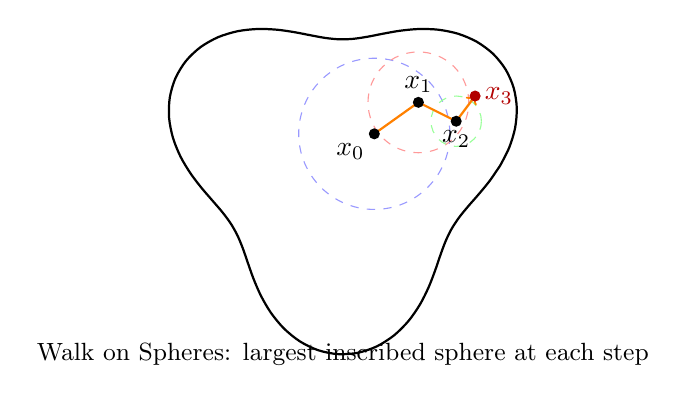
\begin{tikzpicture}[scale=0.8]
  \draw[thick] plot[smooth,domain=0:360,samples=60] (\x:{2.5+0.5*sin(3*\x)}) -- cycle;
  \coordinate (x0) at (0.5,0.5);
  \coordinate (x1) at (1.2,1.0);
  \coordinate (x2) at (1.8,0.7);
  \coordinate (x3) at (2.1,1.1);
  \draw[blue!40,dashed] (x0) circle (1.2);
  \draw[red!40,dashed] (x1) circle (0.8);
  \draw[green!40,dashed] (x2) circle (0.4);
  \draw[->,thick,orange] (x0)--(x1)--(x2)--(x3);
  \fill (x0) circle (2.5pt) node[below left] {$x_0$};
  \fill (x1) circle (2.5pt) node[above] {$x_1$};
  \fill (x2) circle (2.5pt) node[below] {$x_2$};
  \fill[red!70!black] (x3) circle (2.5pt) node[right] {$x_3$};
  \node[font=\small] at (0,-3) {Walk on Spheres: largest inscribed sphere at each step};
\end{tikzpicture}
\caption{Walk on Spheres: from each interior point, jump to a random point on the largest inscribed sphere.}
\label{fig:walk_spheres}
\end{figure}


\subsection{Usage}
\begin{algorithm}
\caption{Stochastic PDE Solver Usage\label{alg:stochastic_pde_usage}}
\begin{algorithmic}[1]
\State \texttt{from compgeom.mesh.algorithms.stochastic\_pde import WalkOnSpheres, WalkOnStars}
\State \texttt{from compgeom import Point3D}
\Statex
\State \texttt{\# Initialize on a surface mesh}
\State \texttt{wos = WalkOnSpheres(mesh)}
\State \texttt{value = wos.solve\_laplace(Point3D(0.5, 0.5, 0.5), boundary\_func)}
\Statex
\State \texttt{\# Robust gradient estimation}
\State \texttt{wost = WalkOnStars(mesh)}
\State \texttt{grad = wost.solve\_gradient(Point3D(0.5, 0.5, 0.5), boundary\_func)}
\end{algorithmic}
\end{algorithm}

\begin{example}[WoS on a Unit Disk]\label{example:wos_unit_disk}
Consider the Laplace equation $\Delta u = 0$ on the unit disk $\Omega = \{(x,y) : x^2 + y^2 < 1\}$ with boundary data $g(\theta) = \cos(2\theta)$. The exact solution is $u(r, \theta) = r^2 \cos(2\theta)$. To estimate $u(0.5, 0)$ via WoS, we start at $(0.5, 0)$, which has inscribed sphere radius $0.5$. A random walk jumps to a point on this sphere, then from the new position computes its inscribed sphere, and so on until hitting $\partial\Omega$. Repeating for $M = 10{,}000$ walks and averaging the boundary values yields an estimate close to $u(0.5, 0) = 0.25 \cdot 1 = 0.25$, demonstrating the convergence stated in \cref{thm:wos_convergence}.
\end{example}

\begin{remark}
The variance of WoS estimators decreases as $O(1/M)$ where $M$ is the number of random walks. For Laplace's equation, the walk is guaranteed to terminate almost surely for bounded domains. For Poisson's equation, an additional correction term accumulates along each walk, increasing variance.
\end{remark}

\subsection{References}
\begin{itemize}
  \item Sawhney, R., \& Crane, K. ``Monte Carlo Geometry Processing: A Meshless Approach to Geometric PDE.'' \textit{ACM Transactions on Graphics (SIGGRAPH)}, 2020 \cite{sawhney2020}.
  \item Yu, Y., et al. ``Robust Derivative Estimation with Walk on Stars.'' \textit{ACM Transactions on Graphics (SIGGRAPH)}, 2025 \cite{yu2025}.
\end{itemize}

%======================================================================
\section{Wave Kernel Signature}
\label{sec:wave_kernel}

\subsection{Overview}
The Wave Kernel Signature (WKS)\index{Wave Kernel Signature} is a multi-scale geometric descriptor for vertices on a 3D mesh. Like the Heat Kernel Signature (HKS)\index{Heat Kernel Signature}, it is based on the spectral properties of the Laplace--Beltrami operator\index{Laplace--Beltrami operator}. However, while HKS models heat diffusion (essentially a low-pass filter), WKS models the evolution of a quantum particle (wave function) with a specific energy distribution. This makes WKS better at capturing high-frequency geometric details and provides superior performance in non-rigid shape matching \cite{aubry2011}.

\subsection{Definitions}
\begin{definition}[Schr\"{o}dinger Equation]\label{def:schrodinger}
The time-dependent Schr\"{o}dinger equation\index{Schr\"{o}dinger equation} on a Riemannian manifold $(M, g)$ governs the evolution of a quantum state: $i \hbar \frac{\partial \psi}{\partial t} = -\Delta_M \psi$, where $\Delta_M$ is the Laplace--Beltrami operator\cref{def:eikonal} and $\hbar$ is the reduced Planck constant (set to 1 in the geometric setting).
\end{definition}

\begin{definition}[Wave Kernel Signature]\label{def:wks}
The Wave Kernel Signature at vertex $x$ and energy scale $e$ is defined as
$$W(x, e) = \sum_{k=1}^\infty g_e(\lambda_k)^2 \phi_k(x)^2$$
where $\{\lambda_k\}$ and $\{\phi_k\}$ are the eigenvalues and orthonormal eigenfunctions\index{eigenfunction} of the Laplace--Beltrami operator, and $g_e$ is an energy band-pass filter centered at energy $e$ \cite{aubry2011}.
\end{definition}

\begin{definition}[Energy Distribution]\label{def:energy_distribution}
The energy distribution (or spectral filter) $g_e(\lambda)$ is typically a log-normal distribution:
$$g_e(\lambda) = \exp\!\left(-\frac{(\log e - \log \lambda)^2}{2\sigma^2}\right)$$
This ensures that the descriptor is sensitive to relative energy differences, providing a balanced representation of both coarse and fine geometric features \cite{aubry2011,sun2009}.
\end{definition}

\subsection{Theory}
The Wave Kernel Signature $W(x, e)$ at vertex $x$ and energy scale $e$ is defined as the average probability of a particle with energy distribution $g_e$ being found at $x$:
$$W(x, e) = \sum_{k=1}^\infty g_e(\lambda_k)^2 \phi_k(x)^2$$
where $\lambda_k$ and $\phi_k$ are the eigenvalues and eigenfunctions of the Laplace--Beltrami operator.

The filter $g_e$ is usually a log-normal distribution\cref{def:energy_distribution}:
$$g_e(\lambda) = \exp \left( -\frac{(\log e - \log \lambda)^2}{2\sigma^2} \right)$$
This ensures that the descriptor is sensitive to relative energy differences, providing a balanced representation of both coarse and fine geometric features.

The WKS can be interpreted as the diagonal of the spectral projection operator\index{spectral projection} onto the energy band $[e - \sigma, e + \sigma]$. Unlike the HKS (which integrates over all time and thus acts as a low-pass filter), the WKS selects a specific frequency band, making it a ``band-pass'' descriptor that captures geometric information at a particular scale.

\begin{theorem}[WKS Isometry Invariance]\label{thm:wks_isometry}
The Wave Kernel Signature\cref{def:wks} is invariant under isometric deformations\index{isometry invariance} of the surface. That is, if $(M, g)$ and $(M, g')$ are isometric Riemannian manifolds with corresponding eigenpairs $\{(\lambda_k, \phi_k)\}$ and $\{(\lambda_k', \phi_k')\}$, then $W(x, e) = W'(f(x), e)$ for any isometry $f: M \to M'$.
\end{theorem}
\begin{proof}
An isometry preserves the Laplace--Beltrami operator\index{Laplace--Beltrami operator}: $\Delta_{g'} = \Delta_g$ after the pullback by $f$. Hence the eigenvalues $\lambda_k$ are identical ($\lambda_k' = \lambda_k$), and the eigenfunctions satisfy $\phi_k'(f(x)) = \phi_k(x)$. The WKS formula depends only on $\lambda_k$, $g_e(\lambda_k)$, and $\phi_k(x)^2$, all of which are invariant under the isometry. Therefore $W'(f(x), e) = \sum_k g_e(\lambda_k)^2 \phi_k'(f(x))^2 = \sum_k g_e(\lambda_k)^2 \phi_k(x)^2 = W(x, e)$.
\end{proof}

\begin{observation}
While WKS\cref{thm:wks_isometry} is isometry-invariant, it is \emph{not} scale-invariant\index{scale invariance}. Scaling the metric by a constant factor $c$ scales eigenvalues as $\lambda_k \to c^{-2} \lambda_k$, which shifts the WKS along the energy axis. In contrast, the HKS with logarithmic time normalization achieves approximate scale invariance \cite{bronstein2010}.
\end{observation}

\subsection{Algorithm}
\begin{algorithm}
\caption{Wave Kernel Signature\index{Wave Kernel Signature}\label{alg:compute_wks}}
\begin{algorithmic}[1]
\Function{ComputeWKS}{$mesh, num\_basis{=}100, num\_scales{=}100$}
  \State $L, M \gets$ BuildDiscreteLaplacian($mesh$)
  \State $evals, Phis \gets$ \texttt{scipy.sparse.linalg.eigsh}($L, M, k{=}num\_basis, \sigma{=}{-}1e{-}6$)
  \State $e\_min \gets \log(evals[1])$ \Comment{Skip zero eigenvalue}
  \State $e\_max \gets \log(evals[-1])$
  \State $scales \gets$ np.linspace($e\_min, e\_max, num\_scales$)
  \State $\sigma \gets (e\_max - e\_min) / num\_scales \times 7.0$ \Comment{Heuristic width}
  \State $wks \gets$ np.zeros(($num\_vertices, num\_scales$))
  \For{$i, e \in$ enumerate($scales$)}
    \State $weights \gets \exp(-(e - \log(evals))^2 / (2\sigma^2))$
    \State $weights \gets weights / \sum(weights)$
    \State $wks[:, i] \gets (Phis^2) \cdot weights$
  \EndFor
  \State \Return $wks$
\EndFunction
\end{algorithmic}
\end{algorithm}

\begin{example}[WKS on a Sphere]\label{example:wks_sphere}
On a unit sphere, the eigenvalues of the Laplace--Beltrami operator are $\lambda_k = k(k+1)$ for $k = 0, 1, 2, \ldots$, with eigenfunctions being the spherical harmonics $Y_k^m$. Since the sphere is completely symmetric, the WKS at every vertex is identical: $W(x, e) = \sum_{k=0}^{\infty} g_e(k(k+1))^2 \sum_{m=-k}^{k} |Y_k^m(x)|^2$. By the addition theorem for spherical harmonics, $\sum_m |Y_k^m(x)|^2 = (2k+1)/(4\pi)$, which is constant in $x$. Therefore $W$ is the same at all vertices---as expected for a shape with trivial isometry group orbits.
\end{example}

\subsection{Parameter Selections}
\begin{itemize}
  \item \textbf{Number of Eigenfunctions ($k$)}: Typically 100--300. More eigenfunctions are needed than for HKS to capture the ``wave'' behavior.
  \item \textbf{Filter Width ($\sigma$)}: Controls the trade-off between spatial and spectral localization.
  \item \textbf{Scale Range}: Usually spans the entire computed spectrum in log-space.
\end{itemize}

\subsection{Complexity}
\begin{itemize}
  \item \textbf{Eigen-decomposition}\index{eigen-decomposition}: $O(N^{1.5})$ for sparse matrices using Lanczos or LOBPCG solvers.
  \item \textbf{Signature Calculation}: $O(N \cdot k \cdot S)$ where $S$ is the number of scales.
  \item \textbf{Space Complexity}: $O(N \cdot S)$ to store the descriptors.
\end{itemize}

\subsection{Usages}
\begin{itemize}
  \item \textbf{Non-Rigid Shape Matching}\index{non-rigid shape matching}: Finding corresponding points between different poses of the same object (e.g., a human walking) \cite{aubry2011}.
  \item \textbf{Shape Retrieval}\index{shape retrieval}: Creating a global descriptor by pooling WKS values across the mesh \cite{bronstein2008}.
  \item \textbf{Symmetry Detection}\index{symmetry detection}: Identifying vertices with similar geometric contexts.
  \item \textbf{Segment Classification}: Training machine learning models to identify parts of a mesh (e.g., ``head,'' ``arm,'' ``leg'').
\end{itemize}

\subsection{Testing Methods and Edge Cases}
\begin{itemize}
  \item \textbf{Isometry Invariance}\cref{thm:wks_isometry}: Verify that WKS is identical for a mesh in two different isometric poses.
  \item \textbf{Scale Invariance}: WKS is NOT naturally scale-invariant (unlike HKS with normalization). Test how it behaves when the mesh is scaled.
  \item \textbf{Locality}: Verify that WKS correctly identifies high-curvature regions (like fingertips or nose) as having distinct signatures.
  \item \textbf{Low Resolution}: Ensure the signature remains stable even on coarse triangulations.
  \item \textbf{Spectral Truncation}: Observe how the descriptor quality degrades as the number of basis functions $k$ is reduced.
\end{itemize}

\subsection{References}
\begin{itemize}
  \item Aubry, M., Schlickewei, U., \& Cremers, D. (2011). ``The wave kernel signature: A quantum mechanical approach to shape analysis.'' \textit{ICCV Workshops} \cite{aubry2011}.
  \item Sun, J., Ovsjanikov, M., \& Guibas, L. (2009). ``A concise and provably informative multi-scale signature based on heat diffusion.'' \textit{Computer Graphics Forum} \cite{sun2009}.
  \item Bronstein, M.\,M., \& Kokkinos, I. (2010). ``Scale-invariant heat kernel signatures for non-rigid shape retrieval.'' \textit{CVPR} \cite{bronstein2010}.
  \item Wikipedia: Spectral shape analysis.
\end{itemize}
